%%%%%%%%%%%%%%%%%%%%%%%%%%%%%% -*- Mode: Latex -*- %%%%%%%%%%%%%%%%%%%%%%%%%%%%
%% 09-07.tex --      IEEE Service Cup Paper
%% Author          : Philip Johnson
%% Created On      : Mon Sep 23 11:52:28 2002
%% Last Modified By: Philip Johnson
%% Last Modified On: Tue Jan 27 13:23:50 2009
%%%%%%%%%%%%%%%%%%%%%%%%%%%%%%%%%%%%%%%%%%%%%%%%%%%%%%%%%%%%%%%%%%%%%%%%%%%%%%%
%%   Copyright (C) 2009 Philip Johnson
%%%%%%%%%%%%%%%%%%%%%%%%%%%%%%%%%%%%%%%%%%%%%%%%%%%%%%%%%%%%%%%%%%%%%%%%%%%%%%%
%% 

%% Home page: http://iscc.servicescomputing.org/2009/
%% We are applying to the ``Service Computing Contest'' (for university professors/projects)

%% Should show how Hackystat explores ``new frontiers'' in SOA development.
%% 8 page limit for paper.
%% At most five students plus one professor.
%% Due date: February 20, 2009.  
%% Conference: July 7-10, 2009, Los Angeles.

%% Paper ID: 1122, http://confhub.com/MyPapers.php?cid=66

%% For ``peer review mode'', do:
%%   \documentclass[conference,compsoc,peerreview]{IEEEtran}
%% and
%%   \IEEEpeerreviewmaketitle  (after the abstract).

\documentclass[conference,compsoc,peerreview]{IEEEtran}
\usepackage[final]{graphicx}
\usepackage{cite}
\usepackage{url}
% uncomment the % away on next line to produce the final camera-ready version
% and uncomment the \thispagestyle{empty} following \maketitle
%\pagestyle{empty}

\begin{document}

\title{Experiences with Hackystat \\ as a service-oriented architecture}

\author{Philip M. Johnson \\
        Shaoxuan Zhang \\
        Pavel Senin \\
\em  Collaborative Software Development Laboratory \\
      Department of Information and Computer Sciences \\
      University of Hawai'i \\
      Honolulu, HI 96822 \\
      johnson@hawaii.edu \\
}


\maketitle
\IEEEpeerreviewmaketitle
%\thispagestyle{empty}

\begin{abstract}  % 200 words
Hackystat is an open source framework for automated collection and analysis
of software engineering process and product data.  Hackystat has been under
development since 2001, and has gone through eight major architectural
revisions during that time.  In 2007, we performed the latest architectural
revision, whose primary goal was to reimplement Hackystat as a
service-oriented architecture (SOA).  Hackystat Version 8 has now been in
public release for over a year, and this paper reports on our experiences:
the motivations that led us to reimplement the system as a SOA, the
benefits we have experienced from that conversion, and the new challenges
we now face as a result.
\end{abstract}


\section{Introduction}
\label{sec:intro}

Software engineering measurement is a compelling practice in principle. By
gathering data on the structure and quality of code, as well as the
behaviors of the developers as they build it, one can imagine obtaining
useful insight into the current state of development, better estimates of
what lies in store for the future, and ideas on how to improve current
practices and work artifacts.

The reality is that software engineering measurements are difficult to
obtain and difficult to interpret. To the extent that measurements are made
manually, this incurs overhead on the development staff which might seem
expendible when the schedule is tight.  Even when measurements are made,
useful insight and action is often difficult to obtain.  Is test case coverage of 70\%
good, bad, or someplace in between? Even if everyone agrees it is bad, what
exactly should be done, if anything?

Since 2001, we have been developing an open source framework for automated
collection and analysis of software engineering process and product data
called Hackystat (\url{http://www.hackystat.org/})
\cite{csdl2-06-06,csdl2-02-07}.  The goal of Hackystat is to provide an
extensible mechanism that can radically reduce the overhead associated with
collection of a wide variety of software engineering data, along with a
sophisticated toolkit of analyses that can facilitate useful
interpretation.  Over the years, Hackystat has been used in a wide variety
of application areas, including: classroom pedagogy \cite{csdl2-03-12},
inference of test-driven design practice \cite{csdl2-06-13}, software
engineering of high performance computing systems \cite{csdl2-06-08}, and a
telemetry-based approach to software measurement trend definition and
display \cite{csdl2-04-11}.

The Hackystat Framework is intended to be generic: it strives to be neutral
with respect to the platform, programming language and environment,
development process, and application domain.  We have not found this to be
a simple goal, and the architecture of Hackystat has undergone eight
significant revisions since 2001 in response to new application demands
upon the framework.

One of the most significant architectural revisions of all is the most
recent one, which occurred in 2007 when we migrated the Hackystat Framework
from a traditional client-server web application architecture to a
service-oriented architecture (SOA).  This required eight months of
development and a rewrite of most of the system (which by that time had
grown to approximately 350,000 lines of code).  

There are several reasons why Hackystat is an interesting case study in
service oriented architectures.  First, it is a mature and non-trivial
system whose entire source code is available and whose conversion to SOA
was motivated by concrete design issues.  Second, it appears to be unique
among software engineering data collection and analysis systems with
respect to its architecture.  Other systems similar to Hackystat (including
SixthSense Analytics, Programeter, Devcreek, SonarSource, ElectroCodeoGram,
and EPM) have a client-server architecture.  Finally, the Hackystat
architecture implements a carefully designed combination of distributed
computation, caching, and pre-fetching that provides flexibility and
scalability without performance degradation for common analyses.

The SOA version of Hackystat has been in public release for approximately
one year, and this has given us sufficient time to start to understand the
changes, both positive and negative, that have resulted from this move.
Section \ref{sec:motivation} discusses the shortcomings of our prior
Hackystat architecture which led us to reimplement the system in a
service-oriented manner.  Section \ref{sec:soa} introduces our current
service-oriented architecture and its features.  Section
\ref{sec:discussion} presents our experiences, both positive and negative,
with the SOA implementation.  Section \ref{sec:conclusion} summarizes our
conclusions and outlines some of our future architectural directions.


\section{Motivation for the Hackystat SOA architecture}
\label{sec:motivation}

Hackystat architectural design decisions has always followed an ``agile''
approach of implementing ``the simplest thing that could possibly work''.
Since 2001, this has resulted in eight significant re-designs of the system
as it outgrew the constraints imposed by the previous architecture.  Some
might view this as a process-level bug, but we view it as a feature: we
could never have predicted in advance which application areas Hackystat
would be used in and the specific architectural pressures they would
create.  As a result, Hackystat's current implementation as a SOA
architecture is not based upon SOA being the current ``hot'' architecture,
but rather as a response to specific issues we were facing with the
previous version and the hope that SOA could address them.

To understand the costs and benefits of Hackystat Version 8, it is
important to know a little bit about Hackystat Version 7.  First, by
Version 7, Hackystat had expanded to support software engineering data
collection and analysis in a variety of very different domains, including
Java-based classroom instruction, C-based high performance computing, Java
and Visual Studio-based test driven design inference, build system analysis
for NASA, a ``continuous'' approach to the Goal-Question-Metric paradigm,
and others.  To support sharing of overlapping functionality between these
domains, the 350 KLOC in the system were broken down into approximately 70
different modules.  While it was possible to build a release of Hackystat
containing all of these modules (and we did so for testing purposes), we
found that any particular domain of application was much better served by
supporting Hackystat ``configurations'', or builds of the system containing
a subset of all possible modules.

Figure \ref{fig:configurations} illustrates Hackystat modules, subsystems,
and configurations in Version 7.  It shows samples of modules (such as
``Standard'', ``HPC Experiment'', etc.) from two configurations: HPC and
Classroom.  Although only 10 modules are shown in the figure due to space
limitations, both configurations contained over 30 modules in reality.
Modules are assigned to one of four ``subsystems'' depending upon their
functionality: the ``Sensor'' subsystem contains modules providing software
``plugins'' to various tools; the ``SDT'' subsystem contains
implementations of structured sensor data called``sensor data types'', the
``Core'' subsystem provides basic client and server-side infrastructure,
and the ``App'' subsystem contains domain-specific analyses and user
interface facilities.

\begin{figure*}[ht]
  \center
  \includegraphics[width=0.7\textwidth]{configurations5.eps}
  \caption{Two example Version 7 configurations}
  \label{fig:configurations}
\end{figure*} 


\subsection{Subsystem configuration binding time}

Hackystat consists of a number of subsystems that can be flexibly composed to support different application requirements.  As the number of application areas supported by Hackystat grew, providing a single ``kitchen sink'' version became unwieldy.  We thus began building different configurations of the system with differing combinations of components that would specialize Hackystat to different application areas (classroom use, high performance computing experimentation, TDD, etc.) 

This configuration had to occur at system build time, which produced a number of problems.

\subsection{Complexity of build}

Once Hackystat outgrew a single subsystem configuration, the complexity of the build process increased dramatically. We needed to implement a custom build system on top of Ant with its own dependency resolution mechanism in order to support a context-sensitive build process that would produce a single binary.  

This custom build process dramatically increased the barrier to entry for new Hackystat developers, as they now had to learn a custom build system in order to add their own extensions to the framework.

\subsection{Lack of access to ``intermediate'' analyses}

In the early stages of Hackystat development, sensor data was sent to a web server, which performed relatively simple analyses over that data before presenting that data to the user in a web page.   As the complexity of our analyses increased, we found it useful to brek them down into ``pipelines''.  For example, to obtain telemetry (trend) data, the raw sensor data would first be analyzed into intermediate objects called ``DailyProjectData'', which would then be composed in various ways by the telemetry mechanism to produce the trends of interest.  The Test-Driven Design analysis would first organize the raw sensor data into ``episodes'' which would then be classified as TDD conformant or not. 

The resulting problem is that while analyses were decomposed into pipelines, access was still monolithic in terms of the web server interface. It was difficult to get access to these intermediate analyses, which were often useful and interesting in their own right. 

\subsection{Server-side implementation language specificity}

The Hackystat framework is designed to be generic within the domain of collection and analysis of software engineering process and product data.  It should run on all platforms, support sensors for arbitrary software development tools and languages, and support analyses for a wide variety of process and product measurement types. 

The same language ``neutrality'' did not hold true when it came to the framework itself.  Client-side sensors could (and were) written in a variety of languages: Java, C\#, Emacs Lisp, etc. The server, however, was a Java web application, and all analyses and user interfaces were required to be written in Java and conform to the Hackystat web interface structure.  

\subsection{UI rigidity}

To simplify UI development, the system provided a high-level API for adding
new commands to the Hackystat web application interface.  This reduced the
amount of code required for the development of any individual command, but
at two costs: developers now had to learn a Hackystat-specific UI API, and
(most importantly) the UI to Hackystat was ``frozen'' in a single design
and there was no practical way to experiment with alternative user
interfaces.

\subsection{Cache thrash}

In the Telemetry application, it was not uncommon to periodically request an analysis that might display 30 or 40 trend lines over the last several months, which would potentially involve the processing of hundreds of thousands of raw sensor data instances. However, many of those trend lines might require access to the raw same sensor data, and many of the trend line components might involve computations that were performed previously the last time the analysis was requested.  

We quickly discovered that the naive implementation of telemetry could easily take several hours to perform an analysis, but with the implementation of caching, we could reduce response time to seconds or minutes.  

Unfortunately, caching created its own problems. The ``pipeline'' nature of analyses like Telemetry meant that we needed to introduce caches at multiple levels.  The sheer size of the Hackystat sensor data repository meant that we could not simply cache everything; we needed to limit the sizes of the various caches.  As the number of caches increased, we started to see evidence of ``cache thrash'': two caches would appear to be discarding objects just as another cache would be requesting them. We found this to be an extremely difficult performance issue to debug.


\section{Hackystat as SOA}
\label{sec:soa}

This section will present the Hackystat SOA architecture.

\section{Pros and cons of SOA}
\label{sec:discussion}

Here we discuss how the SOA architecture addressed all of the issues we encountered in Section \ref{sec:motivation}, and what new issues we are confronting. 

Pro: Restart a single service without bringing down entire system.

Con: Loss of compile-time structural consistency checking for sensor data types.

\section{Conclusions}
\label{sec:conclusion}

Conclusions and future directions. 


\bibliographystyle{IEEEtran}
\bibliography{tdd,zorro,csdl-trs,hackystat,psp}
\end{document}











